\chapter{Analytická část}\label{chap:anal}

V této kapitole se budu věnovat analýze aktuálního stavu testovací knihovny a možnostech jejího rozšíření.


\section{Analýza stávajícího stavu knihovny}

Původní testovací knihovna byla výstupem mojí bakalářské práce\cite{bakalarka} dokončené v roce 2021. Cílem této knihovny byla automatizace testů verifikace průmyslové komunikace a integrace do kontinuálního testování na Azure DevOps serveru. 

Knihovna rozlišuje tři druhy účastníků testování:

\begin{description}
    \item[Testovací služba] Služba, která řídí testovací běh.
    \item[Testované zařízení] Hlavní účastník testování, který běží na jiném zařízení, než ze kterého běží testovací služba. 
    \item[Testovací partner] Zařízení, které simuluje nějaké testované zařízení. Toto zařízení běží na stejném zařízení, jako testovací služba. 
\end{description}

Ideou knihovny je, že testovací služba, která řídí a synchronizuje běh na všech zúčastněných zařízení, je spouštěna automatizovaně za pomoci Azure DevOps serveru v Azure Pipelines. Společně s ním je spuštěn i vyvíjený produkt, který chceme otestovat, v tomto kontextu nazýván jako testované zařízení. Testované zařízení se následně připojí k testovací službě a po úspěchu této fáze započne samotné testování. 

Pro každý test lze definovat další účastníky testování - testovací partnery. Tito testovací partneři běží pouze po dobu daného testu a po dokončení testu zaniknou. Hlavní úlohou těchto zařízení je simulace protistrany při komunikaci. 

Ukázka možného propojení všech účastníků testování můžeme vidět na obrázku \ref{fig:bp_devicemodel}. Jak zde je vidět, testovací partneři a testovací služba běží na jednom zařízení, takzvaném agentovi, na kterém je primárně spouštěno celé testování. Vlevo dole je vidět testované zařízení SIMATIC ET 200SP, které je propojeno s agentem. Vpravo dole můžeme vidět PLC, které pouze znázorňuje možnost propojení s dalšími externími zařízeními.

\begin{figure}[htbp]
    \centering 
    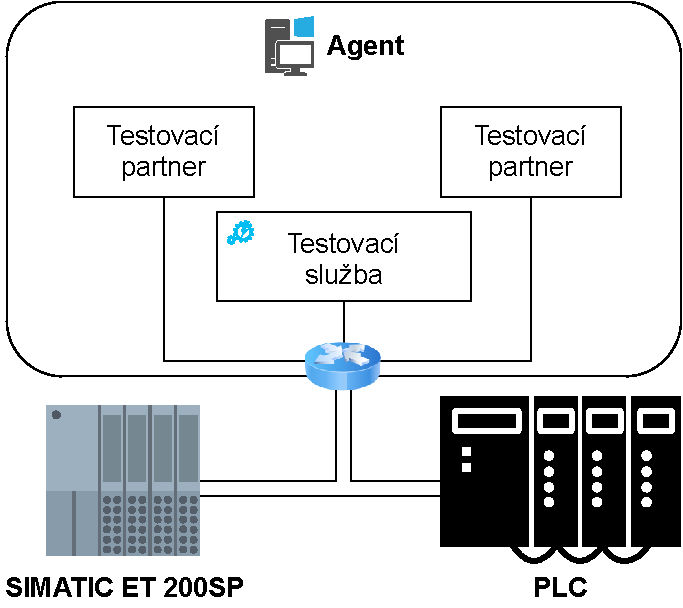
\includegraphics[width=0.97\textwidth]{assets/img/bp_assets/devicemodel.pdf}
    \caption{Ukázka možného propojení účastníků testování v původní knihovně}
    \source{\cite{bakalarka}}
    \label{fig:bp_devicemodel}
\end{figure}


\subsection{Integrace do testovaného zařízení}

K tomu aby mohla být knihovna použita na zařízení, které je testováno, tak je zapotřebí nejdříve implementovat rozhraní pro testované zařízení. Implementací rozhraní definujeme primárně všechny potřebné funkce pro vytvoření spojení mezi testovaným zařízením a testovací službou. Zároveň definujeme funkci pro získávání jednotlivých testů. 

Tyto testy rovněž dodržují jednotnou podobu pomocí rozhraní testu. Toto rozhraní definuje tři fáze testu:

\begin{enumerate}
    \item Příprava na testování -- definování potřebných struktur, inicializace.
    \item Testování -- provedení samotného testu.
    \item Úklid po testu -- uvolnění využitých zdrojů a uvedení zařízení do původního stavu.
\end{enumerate}

Všechna zařízení musí mít pro provedení daného testu implementované rozhraní pro daný test. Testovací služba následně synchronizuje všechna zařízení, tak aby před započetím další testovací fáze všechna zařízení dokončila fázi předchozí. 

\subsection{Možnosti virtualizace v knihovně}

Původní testovací knihovna definuje již předem zmíněné testovací partnery, kteří jsou virtualizovaní participanti testů, sloužící k simulaci protistrany při testování průmyslové komunikace s testovaným zařízením. Jejich implementace kopíruje implementaci pro testované zařízení. Výhodou je, že k jejich využití je potřeba implementovat pouze samotné rozhraní pro test.

Každý testovací partner má životnost pouze v průběhu testu. To znamená, že před započetím testu je každý testovací partner vytvořen a připojen k testovací službě a následně po dokončení testu ukončen. Toto umožňuju variabilní počet testovacích partnerů pro každý testů.

Knihovna nijak neřeší topologii zapojení jednotlivých zařízení, podstatné pouze je, aby všechna zařízení zúčastněná v testu se byla schopna připojit k testovací službě. 


\section{Možnosti rozšíření virtualizačních prvků}

Po shlédnutí možností virtualizace ve stávající knihovně je vidět, že jsou limitované. Knihovna nepodporuje možnost simulovat jakékoliv zařízení a vůbec neřeší topologii zapojení daných zařízení. Zároveň pro každý test je potřeba implementovat rozhraní testu, tedy na všech zařízeních musí být daný test definován. 

Rozšířením knihovny chceme docílit větší možnosti virtualizace a simulace reálného prostředí. Nová knihovna by tedy měla cílit na

\begin{itemize}
    \item možnost spustit jakékoliv zařízení jako virtualizované,
    \item zapojit tato zařízení dle definované topologie (sériové linky, kruhu, hvězdy).
\end{itemize}


\subsection{Virtualizace zařízení}

